% chapter7.tex -- Multi-Layer DFS and Processing Faces One by One
% Based on the author's UGThesis.docx.

\chapter{Multi-Layer DFS and Processing Faces One by One}
\label{ch:multi_layer_dfs}

In this chapter we describe the recursive tree structure that processes faces sequentially, building a global chord set incrementally and backtracking when no compatible triangulation exists for a face. 
We also formalise the pruning strategy introduced in Chapter~\ref{ch:pruning_strategy} in terms of the opposite pairs of generating chords.

\section{Processing Faces Sequentially}
\label{sec:sequential_faces}

Let \(G\) be a biconnected plane graph with \(k\) faces \(F_1, F_2, \dots, F_k\) (the order is arbitrary but fixed). 
We process the faces one after another, maintaining a global chord set \(S\) that contains all chords that have already been added by triangulations of earlier faces.

The overall structure is a \textbf{double-layer tree}:
\begin{itemize}
    \item The outer layer is a recursion over faces: for each face \(F_i\), we explore all its valid triangulations that are compatible with the chords in \(S\) (which come from faces \(F_1, \dots, F_{i-1}\)).
    \item The inner layer is the genealogical tree of triangulations of the current face \(F_i\), as described in Chapter~\ref{ch:cycle_algorithm}, but with additional pruning based on conflicts with \(S\).
\end{itemize}

We denote a triangulation of face \(F_i\) by \(t_{i,j}\), where \(j\) indexes the triangulations of that face in the order they are generated by the DFS of its local genealogical tree.

\subsection{The Double-Layer Tree Structure}
\label{subsec:double_layer}

The exploration proceeds as follows:

\begin{enumerate}
    \item Start with an empty global chord set \(S = \emptyset\) and an empty partial triangulation \(T = \emptyset\).
    \item For face \(F_1\), build its genealogical tree (using the cycle algorithm). 
    For each triangulation \(t_{1,j}\) of \(F_1\):
        \begin{itemize}
            \item Add the chords of \(t_{1,j}\) to \(S\) (temporarily).
            \item Move to face \(F_2\) with the updated \(S\).
        \end{itemize}
    \item For face \(F_2\), build its genealogical tree, but only consider those triangulations that do not create multi-edges with the chords already in \(S\) (i.e., no chord of the triangulation is already in \(S\) unless it is a boundary edge of the face). 
    For each valid triangulation \(t_{2,j}\):
        \begin{itemize}
            \item Add its chords to \(S\).
            \item Move to face \(F_3\).
        \end{itemize}
    \item Continue recursively until the last face \(F_k\). 
    When a complete set of triangulations \(t_{1,j_1}, t_{2,j_2}, \dots, t_{k,j_k}\) has been accumulated without conflicts, the union of all chords forms a valid global triangulation of \(G\). 
    Output this triangulation.
    \item After exhausting all triangulations of the current face, backtrack: remove the chords of that face from \(S\) and try the next triangulation of the previous face.
\end{enumerate}

\begin{figure}[htbp]
    \centering
    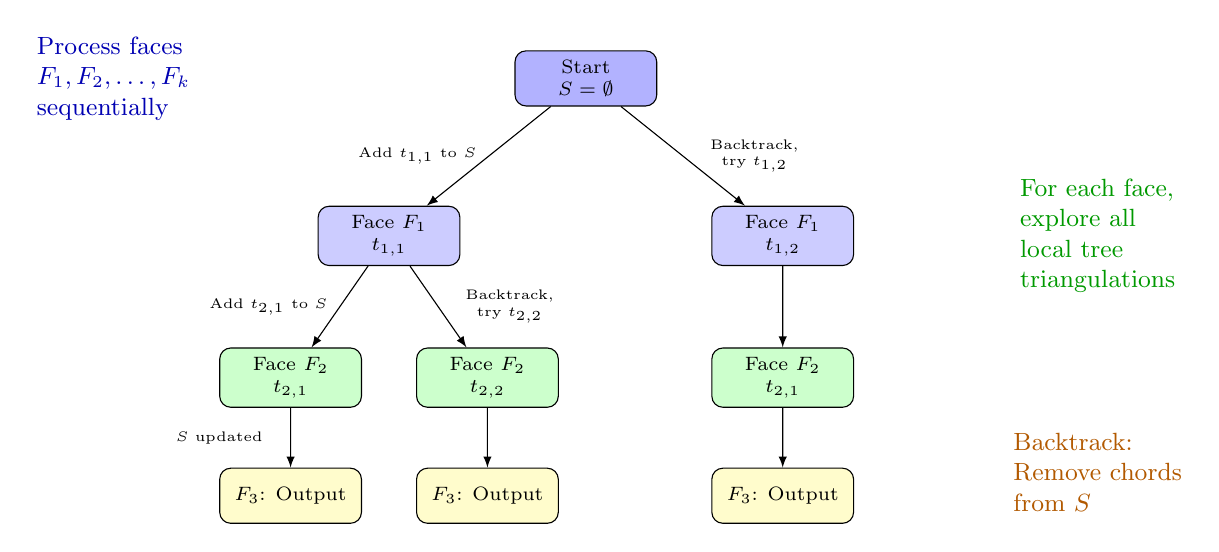
\begin{tikzpicture}[
        level 1/.style={sibling distance=5cm, level distance=2cm},
        level 2/.style={sibling distance=2.5cm, level distance=1.8cm},
        level 3/.style={sibling distance=1.5cm, level distance=1.5cm},
        every node/.style={rectangle, rounded corners, minimum width=1.8cm, minimum height=0.7cm, align=center, font=\scriptsize},
        edge from parent/.style={draw, -latex}
    ]
        \node[draw, fill=blue!30] {Start \\ $S = \emptyset$}
        child {
            node[draw, fill=blue!20] {Face $F_1$ \\ $t_{1,1}$}
            child {
                node[draw, fill=green!20] {Face $F_2$ \\ $t_{2,1}$}
                child {
                    node[draw, fill=yellow!20] {$F_3$: Output}
                    edge from parent node[left, draw=none, font=\tiny] {$S$ updated}
                }
                edge from parent node[left, draw=none, font=\tiny] {Add $t_{2,1}$ to $S$}
            }
            child {
                node[draw, fill=green!20] {Face $F_2$ \\ $t_{2,2}$}
                child {
                    node[draw, fill=yellow!20] {$F_3$: Output}
                }
                edge from parent node[right, draw=none, font=\tiny] {Backtrack,\\ try $t_{2,2}$}
            }
            edge from parent node[left, draw=none, font=\tiny] {Add $t_{1,1}$ to $S$}
        }
        child {
            node[draw, fill=blue!20] {Face $F_1$ \\ $t_{1,2}$}
            child {
                node[draw, fill=green!20] {Face $F_2$ \\ $t_{2,1}$}
                child {
                    node[draw, fill=yellow!20] {$F_3$: Output}
                }
            }
            edge from parent node[right, draw=none, font=\tiny] {Backtrack,\\ try $t_{1,2}$}
        };

        \node[draw=none, font=\small, align=left, blue!70!black] at (-6, 0)
        {Process faces\\$F_1, F_2, \ldots, F_k$\\sequentially};

        \node[draw=none, font=\small, align=left, green!60!black] at (6.5, -2)
        {For each face,\\explore all\\local tree\\triangulations};

        \node[draw=none, font=\small, align=left, orange!70!black] at (6.5, -5)
        {Backtrack:\\Remove chords\\from $S$};
    \end{tikzpicture}
    \caption{Double-layer DFS: outer recursion over faces, inner recursion over triangulations of each face. 
    The global chord set \(S\) is updated when entering a branch (push) and restored when backtracking (pop). 
    Each path from the root to a leaf corresponds to a complete valid triangulation of the graph.}
    \label{fig:double_layer_dfs}
\end{figure}

\subsection{Global Chord Set Management}
\label{subsec:global_chord_set}

The global chord set \(S\) is implemented as a hash set for expected \(O(1)\) insertion, deletion, and membership queries. 
During the DFS:
\begin{itemize}
    \item When we enter a node (i.e., when we commit to a particular triangulation \(t_{i,j}\) of face \(F_i\)), we insert all chords of \(t_{i,j}\) into \(S\) (except the boundary edges of the face, which are already present as edges of \(G\)).
    \item When we backtrack from that node (after exploring all its descendants), we remove those chords from \(S\).
\end{itemize}
This ensures that \(S\) always contains exactly the chords from the current partial triangulation along the recursion path.

\section{Pruning by Opposite Pair of Generating Chords}
\label{sec:pruning_opposite}

We now revisit the pruning condition introduced in Chapter~\ref{ch:pruning_strategy} and express it in terms of the opposite pairs of generating chords.

Recall that in the local genealogical tree of a face with root vertex \(v_r\), a child triangulation is obtained by flipping a generating chord \((v_r, v_j)\). 
The new chord added is the \textbf{opposite pair} \((v_o, v_{o'})\) of \((v_r, v_j)\). 
This new chord does \textbf{not} have \(v_r\) as an endpoint.

\begin{lemma}[Pruning by opposite pair]
    \label{lem:pruning_opposite}
    Let \(T\) be a triangulation of the current face \(F_i\) during the DFS, and let \((v_r, v_j)\) be a generating chord of \(T\) whose opposite pair is \((v_o, v_{o'})\). 
    If \((v_o, v_{o'})\) already belongs to the global chord set \(S\) (i.e., it was created by a previous face \(F_p\) with \(p < i\)), then the child triangulation \(T' = \text{Flip}(T, (v_r, v_j))\) is invalid, and furthermore the entire subtree of the genealogical tree rooted at \(T'\) contains only invalid triangulations.
\end{lemma}

\begin{proof}
    After flipping, the chord \((v_o, v_{o'})\) is present in \(T'\). 
    Because it does not have the root vertex \(v_r\) as an endpoint, Lemma~\ref{lem:persistence} guarantees that \((v_o, v_{o'})\) persists in all descendants of \(T'\) in the local genealogical tree. 
    Since \((v_o, v_{o'}) \in S\) and chords from previous faces are permanent, every descendant would contain a multi-edge. 
    Hence the entire branch is invalid and can be safely pruned.
\end{proof}

Therefore, when generating children of a triangulation \(T\), we only flip those generating chords \((v_r, v_j)\) for which the opposite pair is not already in \(S\). 
All other generating chords are skipped (their branches are pruned at the root).

\begin{figure}[htbp]
    \centering
    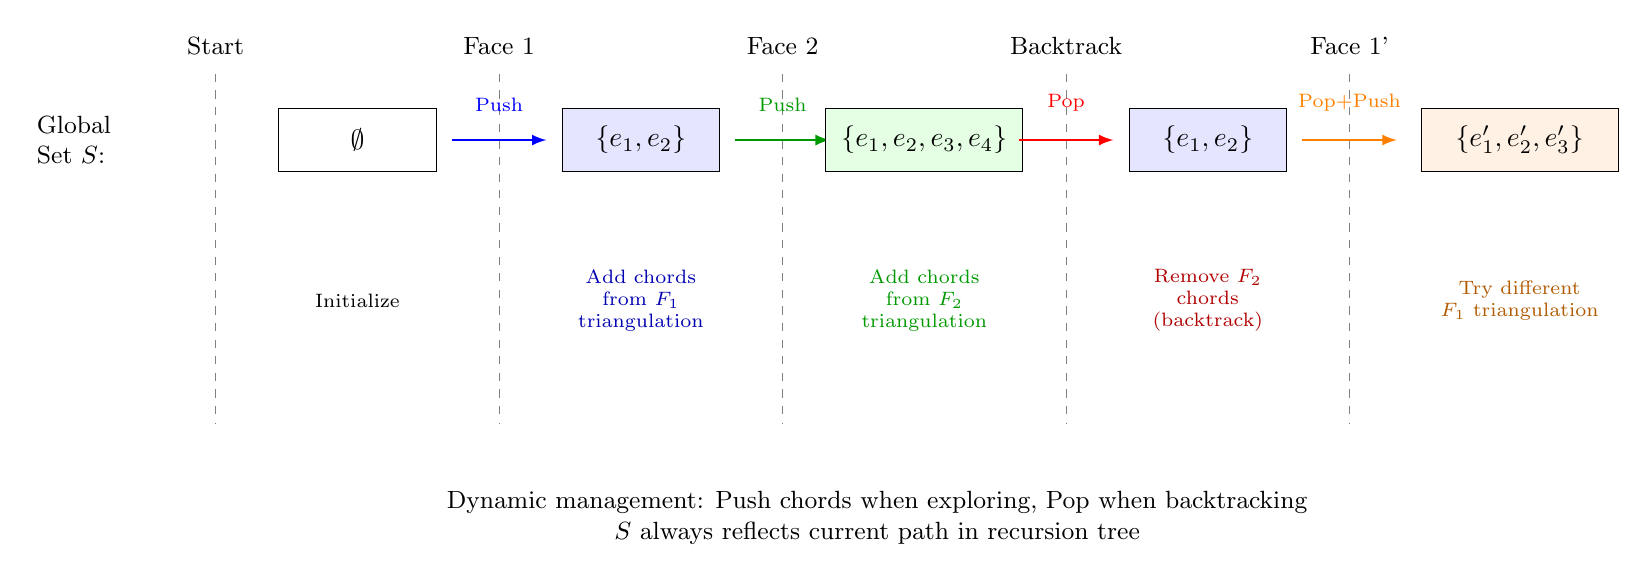
\begin{tikzpicture}[scale=1.2]
        % Timeline representation
        \foreach \x/\label in {0/Start, 3/Face 1, 6/Face 2, 9/Backtrack, 12/Face 1'} {
            \node[font=\small] at (\x, 3.5) {\label};
            \draw[dashed, gray] (\x, 3.2) -- (\x, -0.5);
        }

        % S contents over time
        \node[draw=none, font=\small, align=left] at (-1.5, 2.5) {Global\\Set $S$:};

        % Empty at start
        \node[draw, minimum width=2cm, minimum height=0.8cm] at (1.5, 2.5) {$\emptyset$};

        % After Face 1
        \draw[-latex, thick, blue] (2.5, 2.5) -- (3.5, 2.5);
        \node[draw=none, font=\scriptsize, blue, above] at (3, 2.7) {Push};
        \node[draw, minimum width=2cm, minimum height=0.8cm, fill=blue!10] at (4.5, 2.5)
            {$\{e_1, e_2\}$};

        % After Face 2
        \draw[-latex, thick, green!60!black] (5.5, 2.5) -- (6.5, 2.5);
        \node[draw=none, font=\scriptsize, green!60!black, above] at (6, 2.7) {Push};
        \node[draw, minimum width=2.5cm, minimum height=0.8cm, fill=green!10] at (7.5, 2.5)
            {$\{e_1, e_2, e_3, e_4\}$};

        % Backtrack from Face 2
        \draw[-latex, thick, red] (8.5, 2.5) -- (9.5, 2.5);
        \node[draw=none, font=\scriptsize, red, above] at (9, 2.7) {Pop};
        \node[draw, minimum width=2cm, minimum height=0.8cm, fill=blue!10] at (10.5, 2.5)
            {$\{e_1, e_2\}$};

        % Try different Face 1 triangulation
        \draw[-latex, thick, orange] (11.5, 2.5) -- (12.5, 2.5);
        \node[draw=none, font=\scriptsize, orange, above] at (12, 2.7) {Pop+Push};
        \node[draw, minimum width=2.5cm, minimum height=0.8cm, fill=orange!10] at (13.8, 2.5)
            {$\{e_1', e_2', e_3'\}$};

        % Action annotations below
        \node[draw=none, font=\scriptsize, align=center] at (1.5, 0.8) {Initialize};
        \node[draw=none, font=\scriptsize, align=center, blue!70!black] at (4.5, 0.8)
            {Add chords\\from $F_1$\\triangulation};
        \node[draw=none, font=\scriptsize, align=center, green!60!black] at (7.5, 0.8)
            {Add chords\\from $F_2$\\triangulation};
        \node[draw=none, font=\scriptsize, align=center, red!70!black] at (10.5, 0.8)
            {Remove $F_2$\\chords\\(backtrack)};
        \node[draw=none, font=\scriptsize, align=center, orange!70!black] at (13.8, 0.8)
            {Try different\\$F_1$ triangulation};

        \node[draw=none, font=\small, align=center] at (7, -1.5)
            {Dynamic management: Push chords when exploring, Pop when backtracking\\
             $S$ always reflects current path in recursion tree};
    \end{tikzpicture}
    \caption{Dynamic global chord set management. The set \(S\) is updated with push/pop operations during the DFS. 
    Only chords that are not already in \(S\) can be added; otherwise the branch is pruned.}
    \label{fig:global_chord_management}
\end{figure}

\section{Backtracking When No Compatible Triangulation Exists}
\label{sec:backtracking}

During the exploration of the genealogical tree of a face \(F_i\), it is possible that no triangulation (including the root) is compatible with the current global set \(S\). 
In that case, we backtrack to the previous face \(F_{i-1}\) and try its next triangulation.

More formally, the recursive procedure for a face \(F_i\) does the following:
\begin{enumerate}
    \item Find a safe root triangulation \(T_r\) for \(F_i\) (using the algorithm of Chapter~\ref{ch:safe_root}).
    \item If \(T_r\) conflicts with \(S\) (i.e., contains a chord already in \(S\) that is not a boundary edge), then no triangulation of \(F_i\) is compatible; return failure.
    \item Otherwise, explore the local genealogical tree rooted at \(T_r\), but only generate children that satisfy the pruning condition (opposite pair not in \(S\)).
    \item For each valid child, update \(S\) (add its chords), recurse to \(F_{i+1}\), and then backtrack (remove the child’s chords).
    \item After exhausting all valid children, return to the caller.
\end{enumerate}

This backtracking mechanism ensures that we only explore combinations that have a chance of leading to a valid complete triangulation.

\section{Correctness of the Multi-Layer DFS}
\label{sec:multilayer_correctness}

The double-layer DFS is correct because:
\begin{itemize}
    \item The outer recursion enumerates all possible combinations of face triangulations (by the completeness of the cycle algorithm for each face).
    \item The pruning condition (opposite pair already in \(S\)) only eliminates branches that are guaranteed to produce multi-edges (by Lemma~\ref{lem:pruning_opposite}). 
    Hence no valid triangulation is missed.
    \item The use of a global chord set \(S\) with push/pop maintains the invariant that \(S\) always contains exactly the chords from the current partial triangulation along the recursion path.
\end{itemize}

\section{Summary}
\label{sec:multilayer_summary}

We have described a multi-layer DFS that processes faces one by one, maintaining a global chord set \(S\) to detect conflicts. 
The pruning strategy based on opposite pairs of generating chords allows us to safely skip entire subtrees that would inevitably produce multi-edges. 
Backtracking ensures that we explore all compatible combinations without duplicates. 
In the next chapter we address the remaining problem: generating chords themselves may also create conflicts, requiring the concept of a \emph{safe root vertex}.